\section{The Monotone Convergence Theorem and a First Look at Infinite Series}
    \textbf{Definition 2.4.1.} A sequence $(a_n)$ is \textit{increasing} if $a_n \leq a_{n+1}$ for all $n \in \textbf{N}$ and \textit{decreasing} if $a_n \geq a_{n+1}$ for all $n \in \textbf{N}$. A sequence is \textit{monotone} if it is either increasing or decreasing.
    \setcounter{theorem}{1}
    \begin{theorem}[Monotone Convergence Theorem]
        If a sequence is monotone and bounded, then it convergences
    \end{theorem}
    \begin{proof}
        Let $(a_n)$ be monotone and bounded. Let's assume $(a_n)$ is increasing (the decreasing case is handled similarly), and consider the \textit{set} of points $\{a_n: n \in \textbf{N}\}$. Since the series is bounded, this set it also bounded, so using the Axiom of Completeness, we can let
        $$s = \text{sup}\{a_n: n\in\textbf{N}\}$$
        It seems reasonable for $\lim(a_n) = s$
        \begin{center}
            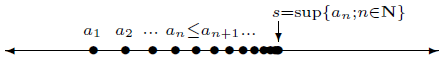
\includegraphics[width=200pt]{sup.png}
        \end{center}
        Let $\epsilon > 0$ be arbitrary. Since $s$ is the least upper bound, $s - \epsilon$ is not an upper bound, so there exists a point in the sequence $a_N$ such that $s - \epsilon < a_N$. Now, since $(a_n)$ is increasing, $a_N \leq a_n$ for all $n \geq N$. Hence,
        $$s - \epsilon < a_N \leq a_n \leq s \leq s + \epsilon$$
        which implies $|a_n - s| < \epsilon$, as desired.
    \end{proof}
    The Monotone Convergence Theorem is useful for infinite series, since it asserts convergences without any mention of the actual limit.
    \textbf{Definition 2.4.3.} Let $(b_n)$ be a sequence. An \textit{infinite series} is a formal expression of the form
    \begin{equation*}
        \sum_{n=1}^\infty b_n = b_1 + b_2 + b_3 + \dots
    \end{equation*}
    We define the corresponding \textit{sequence of partial sums} $(s_m)$ by 
    \begin{equation*}
        s_m = \sum_{n=1}^m b_n = b_1 + b_2 + b_3 + \dots + b_m
    \end{equation*}
    and say the the series $\sum_{n=1}^\infty b_n$ \textit{converges to} $B$ if the sequence $(s_m)$ converges to B. In this case, we write $\sum_{n=1}^\infty b_n = B$.
    \setcounter{theorem}{6}
    \begin{theorem}[Cauchy Condensation Test]
        Suppose $(b_n)$ is decreasing and satisfies $b_n \geq 0$ for all $n \in \textbf{N}$. Then, the series $\sum_{n=1}^\infty b_n$ converges if and only if the series
        \begin{equation*}
            \sum_{n=0}^\infty 2^nb_{2^n}
        \end{equation*}
        converges.
    \end{theorem}
    \begin{proof}
        First, assume that $\sum_{n=0}^\infty 2^nb_{2^n}$ converges. Then the partial sums
        \begin{equation*}
            t_k = b_1 + 2b_2 + 4b_4 + \dots + 2^kb_{2^k}
        \end{equation*}
        are bounded. There exists an $M > 0$ such that $t_k \leq M$ for all $k \in \textbf{N}$. Since $b_n \geq -$, we now that the partial sums are increasing, so we only need to show that 
        \begin{equation*}
            s_m = b_1 + b_2 + \dots + b_m
        \end{equation*}
        is bounded.
        \newline \indent
        Fix $m$ and let $k$ be large enough to ensure $m \leq 2^{k+1} - 1$. Then, $s_m \leq s_{2^{k+1}-1}$ and
        \begin{align*}
            s_{2^{k+1}-1} = b_1 + (b_2 + b_3) + (b_4 + b_5 + b_6 + b_7) + \dots + (b_{2^k} + \dots + b_{2^{k+1} - 1}) \\
            \leq b_1 + (b_2 + b_2) + (b_4 + b_4 + b_4 + b_4) + \dots + (b_{2^k} + \dots + b_{2^k})
            = b_1 + 2b_2 + 4b_4 + \dots + 2^kb_{2^k} = t_k
        \end{align*}
        Thus, $s_m \leq t_k \leq M$, and the sequence $(s_m)$ is bounded. By the Monotone Convergence Theorem, we can conclude that $\sum_{n=1}^\infty b_n$ converges.
        \newline \indent
        Now, if $\sum_{n=0}^\infty 2^nb_{2^n}$ diverges. Fix $m$ and let $k$ be big enough to ensure $m \leq 2^k$. Then, 
        \begin{equation*}
            s_{2^k} = b_1 + b_2 + (b_3 + b_4) + (b_5 + b_6 + b_7 + b_8) + \dots + (b_{2^{k - 1} + 1} + \dots b_{2^k}) \\
            \geq b_1 + b_2 + (b_4 + b_4) + (b_8 + b_8 + b_8 + b_8) + \dots + (b_{2^k} + b_{2^k} + \dots + b_{2^k}) \\
            = b_1 + b_2 + 2b_4 + 4b_8 + \dots + k(b_k) \\
            = b_1 + (t_k - b_1)/2 = (b_1 + t_k) / 2
        \end{equation*}
        So, $s_m > (b_1 + t_k) / 2$, which diverges since $t_k$ diverges so $s_m$ diverges.
    \end{proof}
    \textbf{Corollary 2.4.7} \textit{The series $\sum_{n=1}^\infty 1/n^p$ converges if and only if $p > 1$}